\paragraph{Protocol.} Every challenger is evaluated walk-forward on the snapshot panel of Section~\ref{sec:data}. Test blocks are two calendar months. A model tested in a block is trained only on snapshots from markets that had resolved before the block began, so every training label was public when the test forecasts are made. The baseline is the last traded price. We report the change in Brier score relative to it with an event-level bootstrap over \modelTestMarkets{} test markets, and separately for the last five months (May to September 2026). No feature or setting was chosen on those months. They are not a pristine holdout: we saw scores for the same configurations on those months on an earlier tape half the size, and afterwards changed only the block length and the number of boosting rounds, to reduce compute.

\paragraph{Recalibration.} Platt scaling of the price changes the Brier score by \skillPlattAll{} overall and \skillPlattHold{} in the last five months (positive is better than the price); isotonic regression by \skillIsotonicAll{} and \skillIsotonicHold{}. Category-specific slopes do no better. The miscalibration these methods learn in one period is absent in the next. The quote midpoint, where a quote history exists, scores \skillMidAll{} relative to the last trade.

\paragraph{Learned residuals.} A gradient-boosted model of the residual $y-p$ returns the price itself when its features carry no signal. With price-path, order-flow, and wallet-record features its skill is \skillResFlowAll{} overall and \skillResFlowHold{} in the last five months. Adding the option-model value for price-linked contracts gives \skillResFullAll{} and \skillResFullHold{}. A two-parameter logistic blend of price and option value, which leaves all other contracts at the price, gives \skillBlendAll{} overall and \skillBlendHold{} in the last five months. On the \plMarkets{} price-linked test markets the blend improves on the last trade by \plSkillBlend{}, and on the quote midpoint at the same instant by \plMidBlend{} (change in Brier score \plMidBlendCI{}). Both feature families help out of time, and the option value contributes the larger share. By category the full model improves on the price in crypto thresholds, finance, culture, geopolitics, and mentions markets, is indistinguishable from it in sports, politics, economy, technology, and weather, and is worse on crypto up/down contracts. The pure formula, with nothing fitted, beats the displayed quote midpoint on price-linked contracts by \plMidFair{}: read as a forecast, the formula is better than the screen.

\begin{figure}[t]
\centering
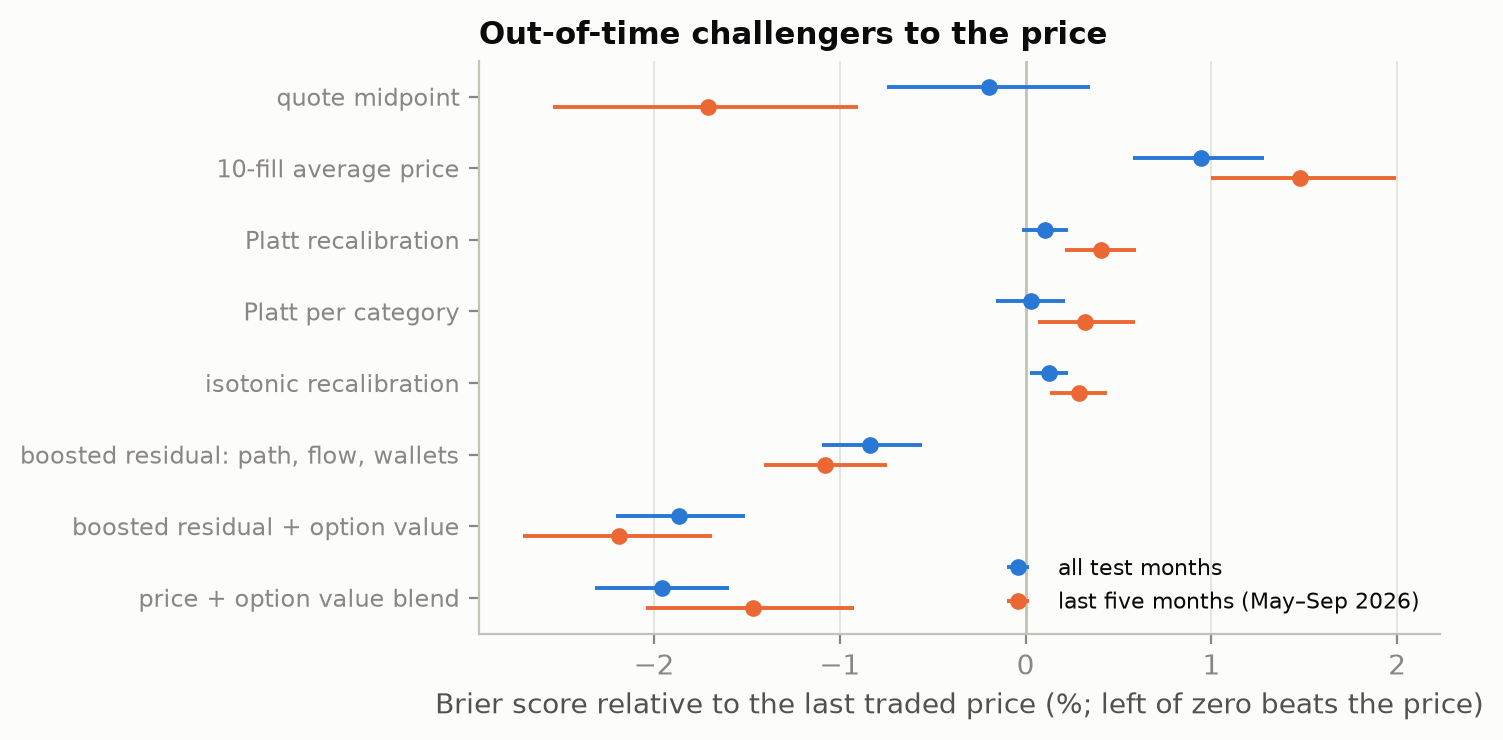
\includegraphics[width=0.56\linewidth]{../results/figures/models.png}\hfill
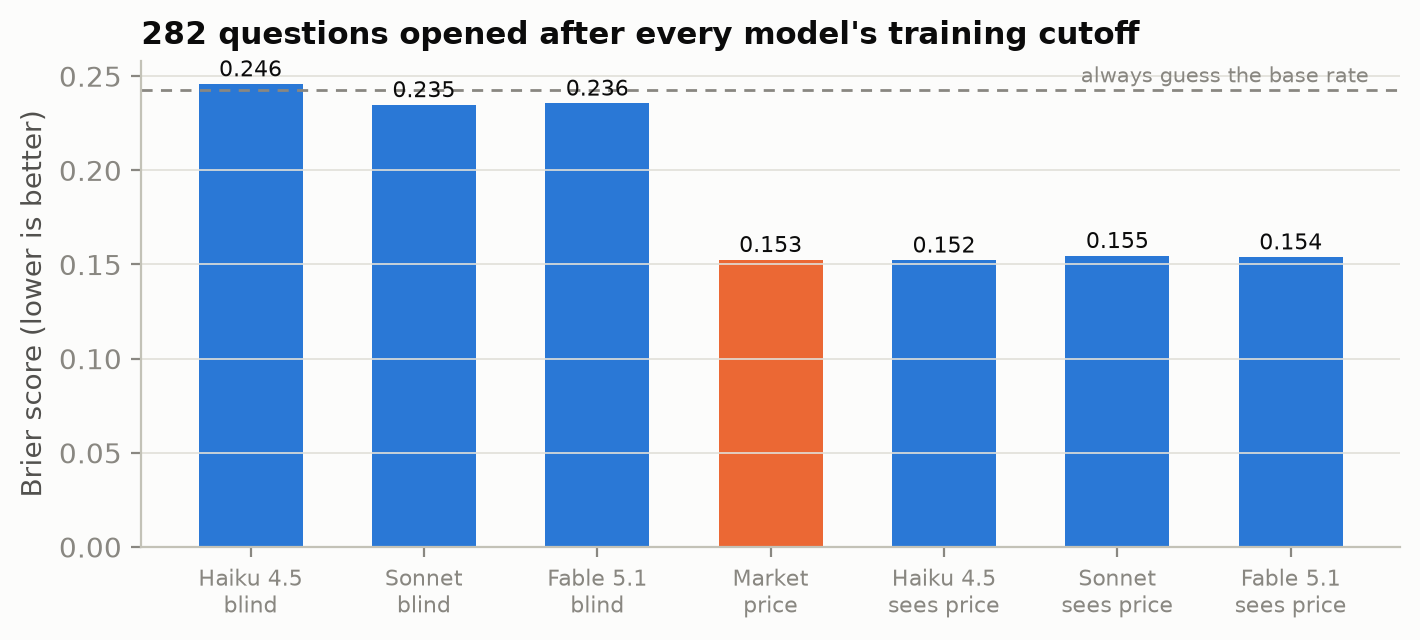
\includegraphics[width=0.42\linewidth]{../results/figures/llm.png}
\caption{Left: Brier score of each challenger relative to the last traded price, walk-forward, with 95\% event-bootstrap intervals. Right: language-model forecasts on questions opened after the models' training cutoffs, with and without the market price in the prompt.}
\label{fig:models}
\end{figure}

\paragraph{Wallet records.} For each fill we compute the taker wallet's realized return on markets that had resolved before the fill. Fills by wallets with no resolved history return \firstTimers{} after fees and fills by seasoned wallets \seasoned{}. Within seasoned wallets, sorting by past return does not sort future return. Our tape covers a sample of markets, so each wallet's record is partial, and this null is weaker evidence than the full-chain result of \citet{gomezcram2026prediction}.

\paragraph{Language models.} We select \llmN{} Yes/No markets that opened after 10 July 2026, one per event, across ten categories, and fix a forecast date at 30\% of each market's scheduled life. Three Claude models (Fable 5.1, Sonnet, Haiku 4.5) receive the question, the resolution rules, and the date, with no tools and no retrieval; each run was verified to have made only the file read and write that the protocol requires. Blind, they score \llmBlindFable{}, \llmBlindSonnet{}, and \llmBlindHaiku{} against a market Brier score of \llmMarket{} and \llmBase{} for a constant base-rate forecast. Shown the market price, they score \llmPriceFable{}, \llmPriceSonnet{}, and \llmPriceHaiku{}, and the weight on the model in a regression that includes the price is not distinguishable from zero. Without news access a language model knows the base rate and nothing the market does not.
